\chapter{Einführung}
%%===========================================================
Auf der ganzen Welt brachten die vergangenen Jahre eine Fortführung des hohen Wachstums des Online Einzelhandels. Der Umsatz stieg im Jahr 2014 um über 20 Prozente weltweit auf fast 840 Milliarden US-Dollar, da Online-Händler weiter in neuen Regionen ausgebaut haben und die physischen Einzelhändler durch E-Commerce in neuen Märkten eingedrungen sind \citep{HanaBen-Shabat2015}. Das schnelle Wachstum des E-Commerce-Marktes hat umfangreiche Forschung angetrieben, um die Meinungen der Konsumenten zum Online Handel besser verstehen zu können \citep{tong2010cross}.

Im Online Handel können die Meinungen der Konsumenten einfach als eine Form der \ac{OCRs} erreicht werden. Mit diesen \ac{OCRs} können eine große Menge an Proben ohne Beschränkung von Zeit und Ort erhalten werden. Anders als traditionelle Umfragen und Fragebogen, sind \ac{OCRs} eine spontane Rückmeldung \citep{lu2015understanding}. Während in den meisten Studien eine Probe von Hunderten Menschen verwendet wird um die Meinungen der Konsumenten zu studieren, könnte ein beliebtes Produkt Tausende von \ac{OCRs} haben. Wegen des Wachstums des E-Commerce werden eine enorme Menge an \ac{OCRs} erzeugt.

Es gibt schon viele Forschungen über \ac{OCRs}. Viele Studien haben die Wichtigkeit der \ac{OCRs} diskutiert, und einige Studien haben schon versucht, die nützliche Information aus den \ac{OCRs} zu extrahieren. In der Mehrheit dieser Studien werden die \ac{OCRs} in zwei Teile unterteilt: der numerische Teil und der schriftliche Teil. Diese Studien fokussieren sich mehr auf den numerischen Teil während der schriftliche Teil von \ac{OCRs} ignoriert wird, trotz der Tatsache, dass der schriftliche Teil mehrere Informationen enthält.

Sentiment Analyse ist ein Teilgebiet des Text Minings, welches den Menschen ermöglicht, die Meinungen der Kunden durch den Text der \ac{OCRs} zu verstehen, ohne manuell den Text durchlesen und zusammenfassen zu müssen. Es ist wichtig, dass die Sentiment Analyse automatisch die Meinungen und die Gefühle der Verfasser der Texte identifizieren kann. Durch die Sentiment Analyse kann man mit den Meinungen der Kunden in dem Text der \ac{OCRs} statistisch rechnen, damit man die Gesamtsituation der Meinungen bewerten kann.

Diese Gesamtsituation ist nützlich, besonders für die kulturübergreifende Forschung. Im Vergleich mit den Situationen aus verschiedenen Ländern kann man die kulturellen Einflüsse auf das Konsumverhalten besser erkennen. Trotz der Tatsache, dass die Unterschiede in der nationalen Kultur das Konsumverhalten beeinflussen könnten, haben die meisten Forschungen über die \ac{OCRs} die Wirkung der Kultur ignoriert \citep{gefen2006need}.

Diese Arbeit macht einen kulturübergreifenden Vergleich zwischen Deutschland und China. Gemeinsam haben die deutschen \acs{B2C}-Mehrkanal-Online- und Versandhandel einen Umsatz von über 49 Milliarden Euro im Jahr 2014. E-Commerce erwirtschaftete mehr als 85 Prozent des gesamten Branchenumsatzes. In Deutschland repräsentierte der Sektor des elektronischen Handels neun Prozent der gesamten Einzelhandelbranche des Landes im Jahr 2014 mit der positiven Tendenz. \citep{Spath2015}

Die chinesischen Online-Käufer sind anspruchsvolle Kunden mit einem großem Markenbewusstsein und Vertrauen in den größten Namen, einschließlich inländischer Marktführer wie Tmall und JD.com sowie internationaler wie Amazon und eBay. In China stellen die chinesischen Käufer im elektronischen Handel ein kulturelles Phänomen dar, vor allem am Ledigen Tag (11. November), der ähnlich wie der Cyber Monday in den USA ist. Alibaba (Plattformbetreiber von Tmall) hat 9,3 Milliarden Dollar Umsatz am Ledigen Tag 2014 gemeldet, was ungefähr sieben Prozent des Gesamtjahresumsatz des Landes entspricht. \citep{HanaBen-Shabat2015}
%%=========================================================
\section{Online Textileinzelhandel in den beiden Ländern} \label{sec:online_kleidung}
%%=========================================================
Dieser Abschnitt stellt die Situationen des Markts von Online Textileinzelhandel in Deutschland und China vor. Diese Vorstellung ist wichtig, man diese Situationen zu wissen, um die Arbeit besser zu verstehen.

Mit mehr als 51 Millionen (94 Prozent der Internetnutzer ab 14 Jahren) digitale Verbraucher im Jahr 2014, genießt Deutschland die größte E-Commerce-Kundenpotenzial in Europa - und ist damit der klare kontinentale Führer \citep{Spath2015}. In ``The 2015 Global Retail E-Commerce Index'' ist Deutschland am fünfth Position \citep{HanaBen-Shabat2015}. 

Kleidung, Elektronische Waren und Bücher gehören zu den beliebtesten Online-Kategorien. 88 Prozente der Befragter sagen, dass sie in den letzten drei Monaten Kleidungen online gekauft haben, während der Weltdurchschnitt 76\% ist. \citep{HanaBen-Shabat2015}

Und die Kategorie ``Bekleidung, Textilien und Schuhe'' hat eine der stärksten Wachstumsraten für den Zeitraum 2011-2014. Die höchsten Umsätze im E-Commerce werden in der Produktkategorien Bekleidungs (11,9 Mrd. EUR), Unterhaltungselektronik (5 Mrd. EUR) und Bücher (4,1 Mrd. EUR) generiert. Als die Abbildung \ref{fig:kleidung_de} gezeigt, werden 42\% Kleidungen in Deutschland online verkauft. \citep{Spath2015} 

\begin{figure}[htb]
	\begin{center}
		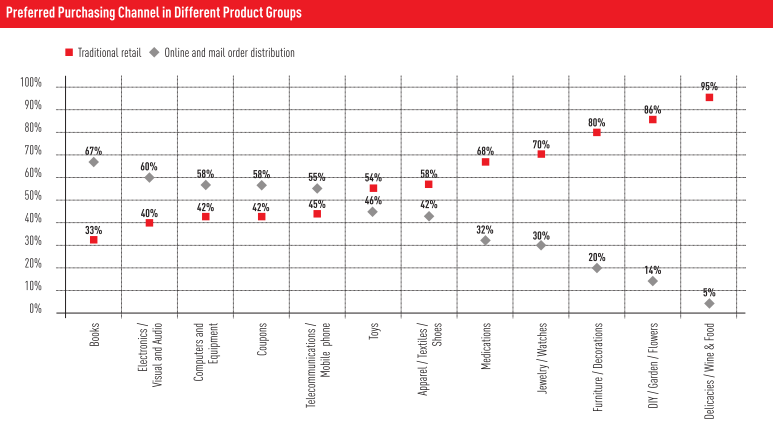
\includegraphics[width = \textwidth]{datensammlung/kleidung_de}
		\caption[42\% Textilien werden in Deutschland online verkauft]{42\% Textilien werden in Deutschland online verkauft(Quelle:\citealp{Spath2015})}
		\label{fig:kleidung_de}
	\end{center}
\end{figure}

China, das weltweit bevölkerungsreichsten Land (fast 1,4 Milliarden Menschen), ist online aktiv. Mehr als ein Drittel der Menschen, die online mindestens einmal pro Woche surfen, sind "ständig verbunden", und 58 Prozenten prüfen das Internet zwei bis vier Mal pro Tag. Verglichen mit Deutschland, ist China am zweiten Position in ``The 2015 Global Retail E-Commerce Index'', nur nach den USA.\citep{HanaBen-Shabat2015}

\begin{figure}[htb]
	\begin{center}
		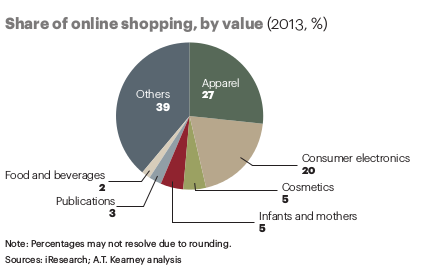
\includegraphics[scale =1.0]{datensammlung/anteil_kleidung_cn}
		\caption[Anteil der Online-Shopping in China]{Anteil der Online-Shopping in China, nach Wert (2013, \%)(Quelle:\citealp{goh2014china})}
		\label{fig:anteil_kleidung_cn}
	\end{center}
\end{figure}

Online-Handel ist die am schnellsten wachsende Einzelhandels für Bekleidung in China \citep{fung2014china}. Abbildung \ref{fig:anteil_kleidung_cn} stellt fest, dass 27\% des Umsatzes in 2013 durch Kleidung verkauft werden, größer als die Kategorie Unterhaltungselektronik. Wie die Abbildung \ref{fig:kleidung_cn} gezeigt, wuchs die gesamte Online-Bekleidungs-Transaktionswert in China deutlich um 42,6\% gegenüber dem Vorjahr um 434,9 Milliarden Yuan (62,1 Milliarden Euro) im Jahr 2013 zu erreichen \citep{fung2014china}.

``Kleidung, Schuhe, Hüte, Taschen und Koffer, Outdoor-Produkte'' sind die beliebtesten Kategorien in Online-Shopping im Jahr 2013 erworben, und diese Kategorie wird von 41,3\% der Frauen und 28\% der Männer inzwischen Top 10 Lieblings Waren in Online-Shopping gewählt \citep{fung2014china}. 97\% der Befragter sagen, dass sie in den letzten drei Monaten Kleidungen online gekauft \citep{HanaBen-Shabat2015}.

\begin{figure}[htb]
	\begin{center}
		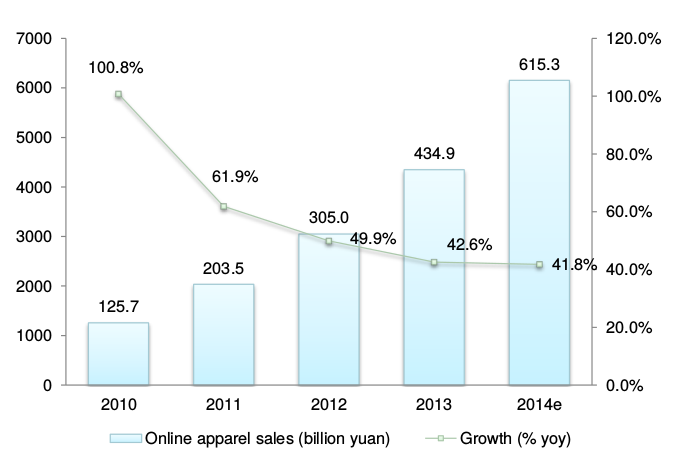
\includegraphics[width=\textwidth]{datensammlung/kleidung_cn}
		\caption[Online Umsatz für Kleidung in China]{Online Umsatz für Kleidung in China, 2010 - 2014(Quelle:\citealp{fung2014china})}
		\label{fig:kleidung_cn}
	\end{center}
\end{figure}

Trotz der Tatsache, dass Online-Textileinzelhandel einer der größten und stark wachsenden Kategorien des elektronischen Einzelhandels ist, gibt es, insbesondere im Bereich \acl{OCRs}, wenig kulturübergreifende Forschung auf diesem Gebiet. \ac{OCRs} können die Kaufentscheidungen der Kunden stark beeinflussen. Zum Beispiel, wollen 40 Prozent der Online Käufer in China unmittelbar ``kaufen oder nicht kaufen'' Beratungen und Bewertungen \citep{HanaBen-Shabat2015}. Deutschland und China, haben große Unterschiede in den Kulturen, und die beiden Länder sind wichtig für die Wirtschaft der Welt, aber es gibt zur Zeit noch keine Forschungen, die über die Unterschiede von Kulturen und \ac{OCRs} zwischen den beiden Ländern diskutiert.
%%===========================================================
\section{Forschungsfragen}
%%===========================================================
Diese Arbeit wird die folgende Forschungsfragen diskutieren:
\begin{enumerate}
	\item Wie sollten die \acl{OCRs} von China und Deutschland sein, basierend auf den theoretischen Grundlagen? 
	\item Welche Unterschiede haben die \acl{OCRs} von China und Deutschland in der Tat durch Sentiment Analyse? 
	\item Welche Unterschiede gibt es zwischen der Praxis und der Theorie? Warum?
	\item Welche Auswirkungen gibt es von diesen Unterschieden der \acl{OCRs} in den beiden Ländern?
\end{enumerate}
%%===========================================================
\section{Die Struktur der Arbeit}
%%===========================================================
Um diese Forschungsfragen zu beantworten, wird die Arbeit in der Struktur geschrieben, die in der Abbildung \ref{fig:struktur} gezeigt wird. Erst werden die deutschen und chinesischen \ac{OCRs} gesammelt, dann werden sie durch die Sentiment Analyse analysiert und die Ergebnisse werden durch statistische Maßnahmen verglichen. Die Unterschiede werden mit den kulturellen Unterschieden diskutiert und begründet. Die Wirkungen dieser Unterschiede werden auch in verschiedenen Sichtweisen diskutiert.

\begin{figure}[htb]
	\centering
	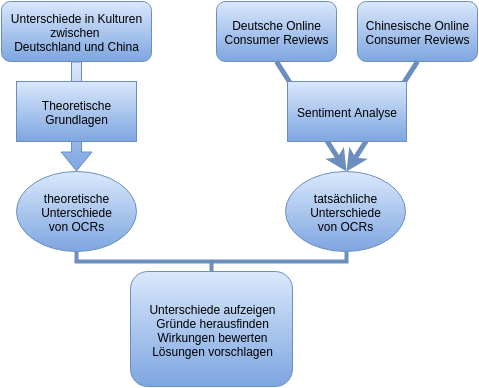
\includegraphics[width=0.85\textwidth]{einfuehrung/struktur}
	\caption[Die Struktur der Arbeit]{Die Struktur der Arbeit (Quelle: Eigene Darstellung)}
	\label{fig:struktur}
\end{figure}

\begin{description}
	\item[Kapitel 2] In Kapitel 2 werden die theoretischen Grundlagen beschrieben. Hier werden erst die \acl{OCRs} vorgestellt, einschließlich des Begriffs und Forschungsstands in der Marketingforschung, der Motive für das Schreiben der \acl{OCRs} und der Wirkungen der \acl{OCRs} im Textileinzelhandel. Danach werden die Definition, der Ablauf, der Kernprozess und der in dieser Arbeit verwendete Algorithmus der Sentiment Analyse eingeführt. Durch die Sentiment Analyse haben die \acl{OCRs} einige statistische Attribute. Dann wird das sechsdimensionale Modell für Deutschland und China von \citeauthor{hofstede2013interkulturelle} vorgestellt, und die Unterschiede zwischen den beiden Ländern werden herausgearbeitet. Die relevanten Forschungsergebnisse im kulturübergreifenden Bereich werden aufgeführt. Basierend auf diesen theoretischen Grundlagen werden vier Hypothesen für die Forschungsfragen aufgestellt. 
	\item[Kapitel 3] Kapitel 3 stellt den Prozess der Datensammlung und Textverarbeitung vor. Die zwei \ac{B2C} Plattformen Amazon Deutschland und Tmall (China) werden als Datenquellen dienen. Vier unterschiedliche Sportbekleidungen von Adidas, Nike und Puma werden als die Untersuchungsobjekte ausgewählt. Diese Untersuchungsobjekte müssen bestimmte Bedingungen erfüllen. Weiterhin werden die technischen Werkzeuge in der Datensammlung vorgestellt und der Datensammlungsprozess aus beiden Plattformen dokumentiert. Nach der Datensammlung werden die Rohdaten bestimmter Verarbeitungen unterzogen und die chinesischen Daten werden durch eine Übersetzungsmaschine auf Deutsch übersetzt, damit die Ergebnisse besser verglichen werden könnten. Die Einflüsse der Übersetzung werden auch in diesem Abschnitt diskutiert.
	\item[Kapitel 4] In diesem Kapitel werden die empirischen Ergebnisse deskriptiv erst gezeigt. Vor der Prüfungen der Hypothesen, muss man erst bestimmen, ob die \acl{OCRs} statistisch normal verteilt sind. Dies ist die Basis dafür, welche Prüfverfahren man für die Hypothesen auswählen sollte. Je nach der Überprüfung der vier Hypothesen wird das Ergebnis gezeigt.
	\item[Kapitel 5] In Kapitel 5 wird erst der Zusammenhang der kulturellen Dimensionen und der Ergebnissen diskutiert, um die Gründe der Unterschiede zwischen China und Deutschland zu entdecken. Und die Motive für das Schreiben der \acl{OCRs} und die Wirkungen der Ergebnisse in Konsumenten-, Unternehmen- und Plattformenbetreiberssicht werden auch diskutiert.  
	\item[Kapitel 6] In diesem Kapitel wird die Arbeit zusammengefasst, und einige Limitationen aus unterschiedlichen Gründen werden aufgestellt. Darüber hinaus wird der Ausblick auf die zukünftigen Forschung geführt.
\end{description} 

